\documentclass[a4paper]{article}

%% Language and font encodings
\usepackage[english]{babel}
\usepackage[utf8x]{inputenc}

\usepackage{booktabs}
\usepackage{tabu}
\usepackage[T1]{fontenc}

%% Sets page size and margins
\usepackage[a4paper,top=3cm,bottom=2cm,left=3cm,right=3cm,marginparwidth=1.75cm]{geometry}

%% Useful packages
\usepackage{amsmath}
\usepackage{graphicx}
\usepackage{titling}
%\usepackage{apacite}
\usepackage[colorinlistoftodos]{todonotes}
\usepackage[colorlinks=true, allcolors=blue]{hyperref}
\usepackage[strings]{underscore}


\title{Modeling and 3D Printing Sea Shells\\
		\large Final Report}
\author{Edward Ye || 100972832}
\date{2019/04/22}

\begin{document}
\maketitle

\begin{abstract}
	Sea shells are an intricate natural object that have been studied and modeled mathematically and computationally. With the advent of consumer 3-D printing, some recent work has gone into create realistic printed versions. This project has attempted to extend techniques of modeling sea shell protrusions, through reaction-diffusion textures, and to ultimately use 3-D printers to fabricate the concrete from the abstract. The techniques involved in generating models and textures are outlined.
\end{abstract}

\tableofcontents

\section{Some Background and Motivation}

Sea shells have interesting patterns which  appear to be readily described by mathematics and computation. Work has already been done to describe aspects of sea shells, from the spiral shape to the color patterns to the protrusions found on the exterior \cite{Galbraith00modelingmurex}\cite{abss}\cite{VANDERHELM1998505}. Recently some work has also gone into the 3D printing of sea shell model \cite{3dprinting-seashells}\cite{bachman-3dprinting}.

The motivation of this project will be to extend the methods of generating the exterior protrusions to be able to mimic a wider variety of shells. Prusinkiewicz and Fowler have modeled periodic ridge and bump patterns and they have also combined multiple generating curves to imitate more intricate shells \cite{abss}. Galbraith et al. have used constructive solid geometry (CSG) to compose different modules to generate a complete Murex Cabritii model. They have proposed the use of reaction-diffusion (RD) to place protrusions algorithmically \cite{Galbraith00modelingmurex}. Intuitively this appears to be a reasonable idea since the protrusion placement of certain shells are something like the placement of spots upon a leopard. Such patterns have already been described as textures using RD \cite{Turk:1991:GTA:127719.122749}.

\pagebreak

\subsection{Main Objective}

An interesting candidate for such a method would be:

\begin{figure}[h]
	\centering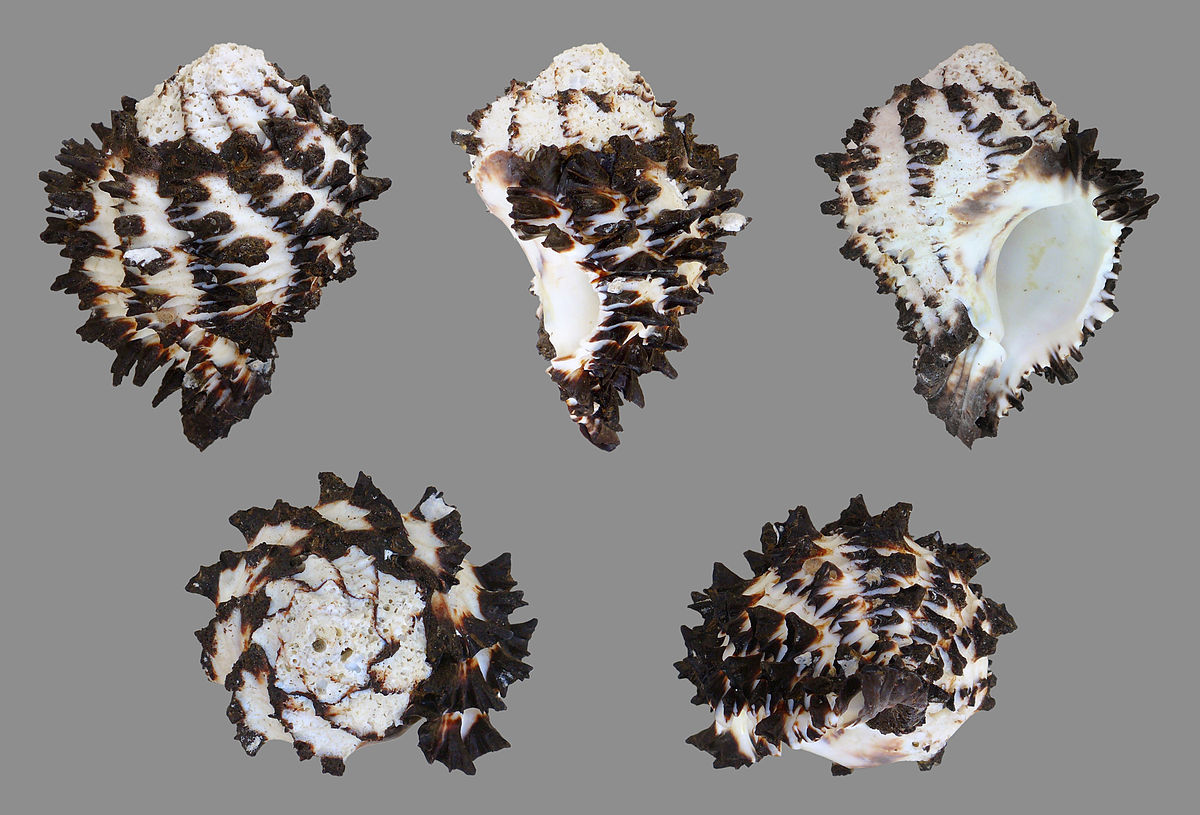
\includegraphics[scale=0.25]{./img/hexaplex_radix.jpg}
	\caption{Hexaplex radix \cite{wikipedia-hexaplex}}
	\label{fig:hexaplex-radix} % Unique label used for referencing the figure in-text
	%\addcontentsline{toc}{figure}{Figure \ref{fig:placeholder}} % Uncomment to add the figure to the table of contents
\end{figure}

The main objective would be to create a model that closely resembles the shell and to 3D print it.

\section{Implicit Surface}

The initial idea was to use a raytracer, such as POV-Ray, to create an implicit surface (isosurface in POV-Ray terminology) that would represent the shell model. The software allows for textures to also act as functions, so that the sum of the implicit equation and the texture function would generate the desired surface. POV-Ray could then generate a point cloud that would form a mesh to be 3-D printed.

\subsection{Logarithmic Spiral}

Shells are modeled by logarithmic spirals. In polar coordinates the logarithmic spiral equation is:

\begin{equation}
	r = Ae^{\alpha \theta}
\end{equation}

Where $A$ shifts the position of the spiral inward or outward, and $\alpha$ multiples the growth rate $(\frac{dr}{d\theta} = \alpha A e^{\alpha \theta} = \alpha r)$.

\begin{figure}[h]
	\centering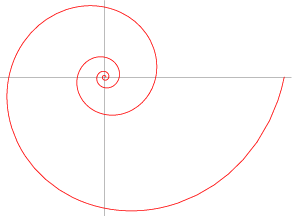
\includegraphics[scale=0.7]{./img/logarithmic-spiral.png}
	\caption{2-D Logarithmic Spiral using equation (1). \cite{logspiral}}
	\label{fig:log-spiral} % Unique label used for referencing the figure in-text
	%\addcontentsline{toc}{figure}{Figure \ref{fig:placeholder}} % Uncomment to add the figure to the table of contents
\end{figure}

\pagebreak

In 3-D Cartesian coordinates (1) can be represented as:

$$ r = \sqrt{x^2 + y^2 + z^2 } $$
$$ \theta = tan^{-1}({\frac{y}{x}}) $$

\begin{equation}
	\sqrt{x^2 + y^2 + z^2 } = A e^{\alpha \cdot tan^{-1}({\frac{y}{x}})}
\end{equation}

Squaring both sides of (2) then gives the implicit equation:

\begin{equation}
	s(x,y,z) = x^2 + y^2 + z^2 - A e^{2 \alpha \cdot tan^{-1}({\frac{y}{x}})} = 0
\end{equation}

\begin{figure}[h]
	\centering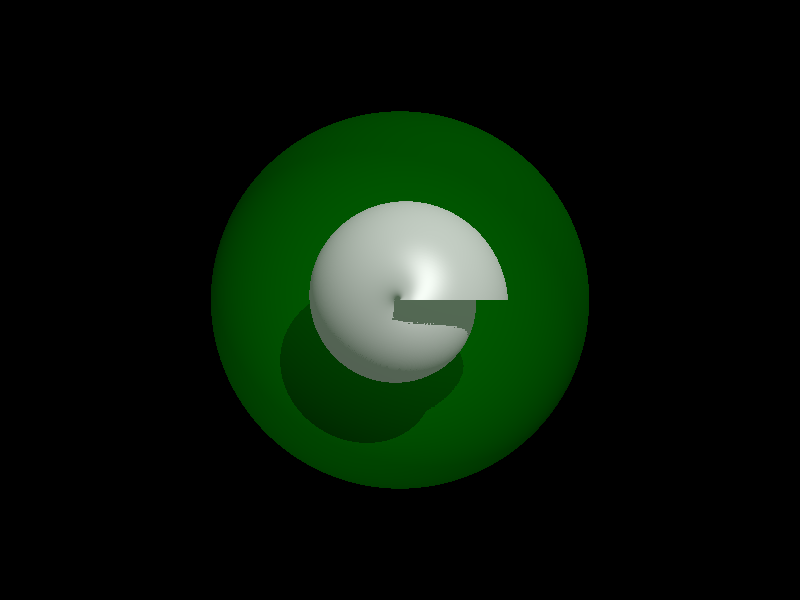
\includegraphics[scale=0.3]{./img/logspiral.png}
	\caption{3-D log spiral generated by \textit{logspiral.pov} using an implementation of equation (3).}
	\label{fig:3d-log-spiral} % Unique label used for referencing the figure in-text
	%\addcontentsline{toc}{figure}{Figure \ref{fig:placeholder}} % Uncomment to add the figure to the table of contents
\end{figure}

If I have some other function, such as $f_{noise}(x,y,z)$, I can add it to equation (3) to get another implicit equation:

\begin{equation}
	s(x,y,z) + f_{noise}(x,y,z) = 0
\end{equation}

\begin{figure}[h]
	\centering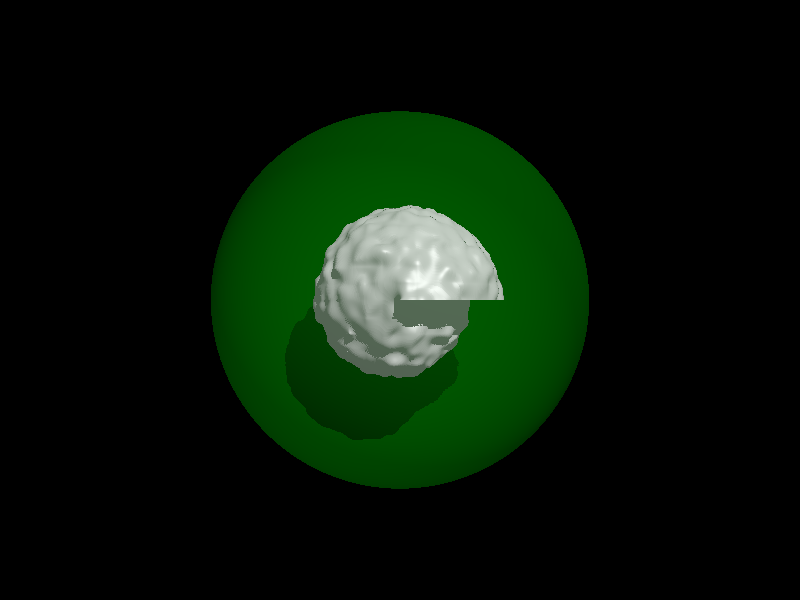
\includegraphics[scale=0.3]{./img/logspiral_noise.png}
	\caption{Equation (4) gives something pretty ugly.}
	\label{fig:3d-log-spiral-noise} % Unique label used for referencing the figure in-text
	%\addcontentsline{toc}{figure}{Figure \ref{fig:placeholder}} % Uncomment to add the figure to the table of contents
\end{figure}

After fiddling around with this for a while it became apparent that the existing parametric equations describing shells could not be easily turned into implicit equations.

\section{Parametric Equations}

Two kinds of parametric equations will be discussed: the first is modified torus used in \cite{povray-seashells}, and the other is a logarithmic spiral with a generating curve used in \cite{JORGEPICADO}.

\subsection{Modified Torus}

The parametric equation for a torus is:

\begin{equation}
	\begin{cases}
		x = (c + a \cdot cos(v)) cos(u)\\
		y = (c + a \cdot cos(v)) sin(u)\\
		z = a \cdot sin(v)\\
	\end{cases}
\end{equation}

for $u,v \in  [0, 2\pi)$.

\begin{figure}[h]
	\centering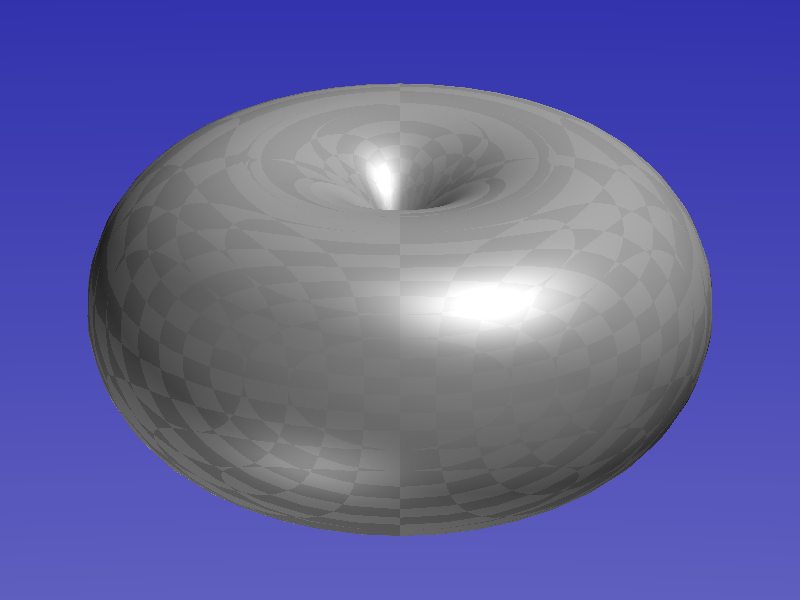
\includegraphics[scale=0.3]{./img/torus.png}
	\caption{Raytraced torus using equation (5).}
	\label{torus} % Unique label used for referencing the figure in-text
	%\addcontentsline{toc}{figure}{Figure \ref{fig:placeholder}} % Uncomment to add the figure to the table of contents
\end{figure}

A simple way to create models resembling sea shells is to form a linear spiral that grows downward as described in \cite{povray-seashells}. The basic equation used is:

\begin{equation}
	\begin{cases}
		w(u) = \frac{u}{2\pi}\\
		x = w(u) \cdot [c + a \cdot cos(v)] cos(N \cdot u)\\
		y = w(u) \cdot [c + a \cdot cos(v)] sin(N \cdot u)\\
		z = w(u) \cdot a \cdot sin(v) + H \cdot [w(u)]^2\\
	\end{cases}
\end{equation}

Where $H$ is the height and $N$ is the number of turns of the spiral. $w(u)$ ensures that the spiral grows linearly from $0$ to $1$, and is used quadratically in the $z$ parameter, so that the height doesn't grow too quickly downward.

\begin{figure}[h]
	\centering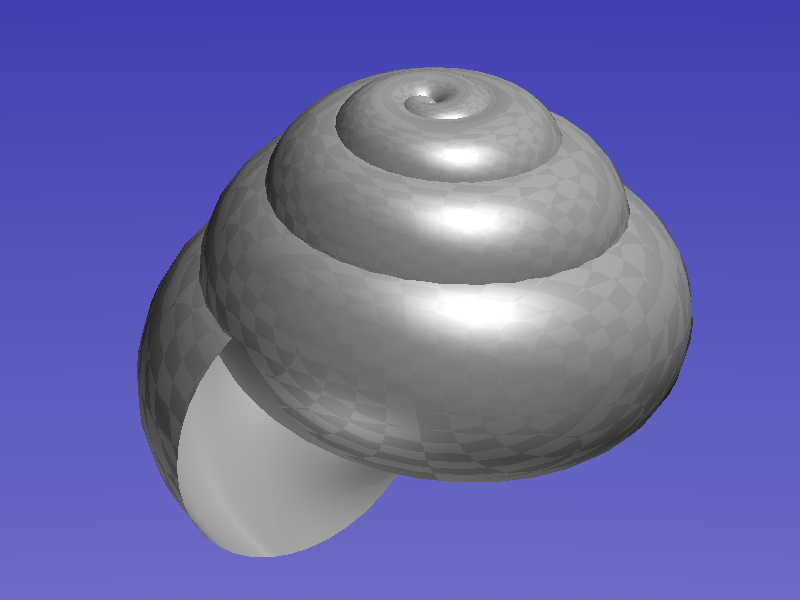
\includegraphics[scale=0.3]{./img/ShellPeriwinkle.png}
	\caption{Periwinkle shell using equation 6, where $a = 1$, $c = 1$, $N = 4.6$ and $H = 2$. \cite{povray-seashells}}
	\label{periwinkle} % Unique label used for referencing the figure in-text
	%\addcontentsline{toc}{figure}{Figure \ref{fig:placeholder}} % Uncomment to add the figure to the table of contents
\end{figure}

\pagebreak

In blender using a XYZ Math Surface (parametric surface) and the modified torus equation, this model was created with the Solidify modifier:

\begin{figure}[h]
	\centering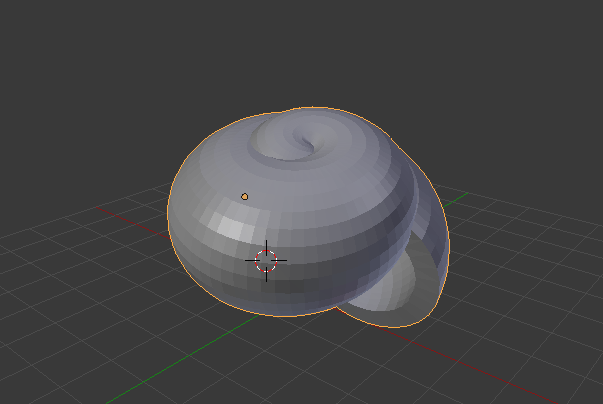
\includegraphics[scale=1.7]{./img/modified_torus_blender.png}
	\caption{Solidified XYZ Math Surface in blender. Exported as \textit{modified\_torus.stl}.
	}
	\label{blender-modified-torus} % Unique label used for referencing the figure in-text
	%\addcontentsline{toc}{figure}{Figure \ref{fig:placeholder}} % Uncomment to add the figure to the table of contents
\end{figure}

\pagebreak

Then it was 3-D printed.

\begin{figure}[h]
	\centering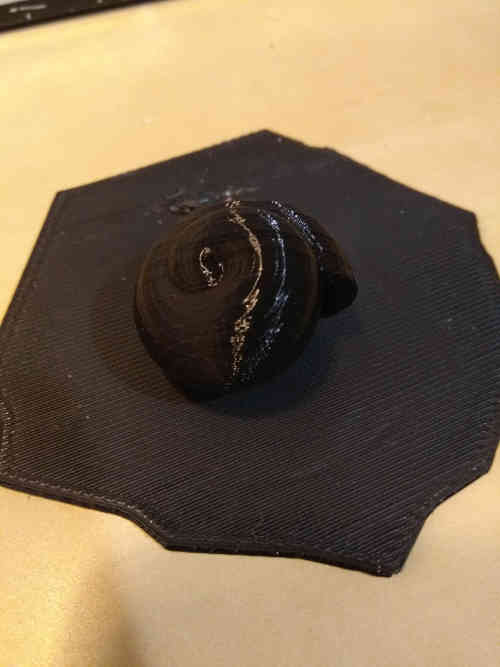
\includegraphics[scale=0.5]{./img/printed_modified_torus.jpg}
	\caption{Printed from \textit{modified\_torus.stl}.}
	\label{3d-printed-torus} % Unique label used for referencing the figure in-text
	%\addcontentsline{toc}{figure}{Figure \ref{fig:placeholder}} % Uncomment to add the figure to the table of contents
\end{figure}

\subsection{Generating Curve} 

The method used in this project is described in detail here \cite{JORGEPICADO}.

\begin{figure}[h]
	\centering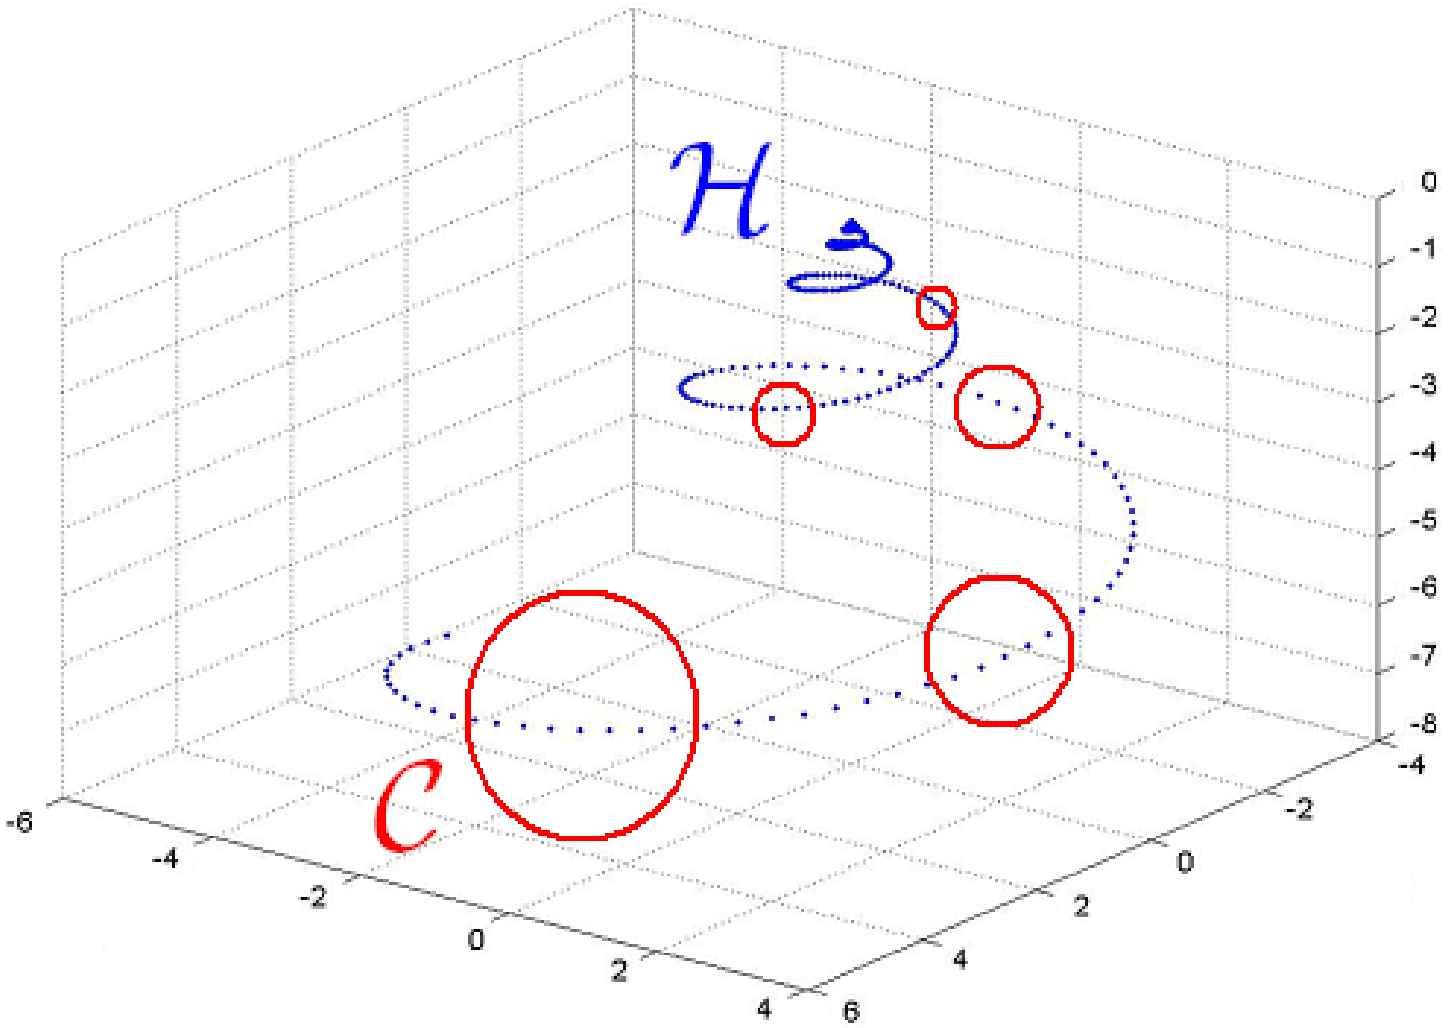
\includegraphics[scale=0.5]{./img/generating_curve.png}
	\caption{$H$ represents the spiral, $C$ the generating curve, which is an ellipse. \cite{JORGEPICADO}}
	\label{3d-printed-torus} % Unique label used for referencing the figure in-text
	%\addcontentsline{toc}{figure}{Figure \ref{fig:placeholder}} % Uncomment to add the figure to the table of contents
\end{figure}

$H$ is a logarithmic spiral, which takes the polar form:

\begin{equation}
	H(\theta) = Ae^{\theta \cot \alpha}
\end{equation}

We get $H(u, v)$ by representing equation (7) in 3-D parametric form:

\begin{equation}
	H(u, v) = 
	\begin{cases}
		x = A sin(v) cos(u) e^{u \cot \alpha}\\
		y = A sin(v) cos (u) e ^{u \cot \alpha}\\
		z = -A cos(u) e^{u \cot \alpha}
	\end{cases}
\end{equation}

\pagebreak

The generating curve $C(u,v,s)$ is an ellipse, with semimajor axis $a$,  semiminor axis $b$, and angle $s$.

\begin{figure}[h]
	\centering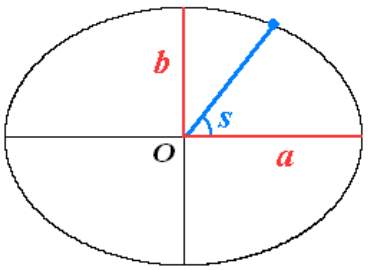
\includegraphics[scale=1.5]{./img/generating_curve_ellipse.png}
	\caption{Elliptical generating curve. \cite{JORGEPICADO}}
	\label{3d-printed-torus} % Unique label used for referencing the figure in-text
	%\addcontentsline{toc}{figure}{Figure \ref{fig:placeholder}} % Uncomment to add the figure to the table of contents
\end{figure}

The parametric elliptical curve equation is:

\begin{equation}
	r_c(s) = \frac{ab}{[(a \cdot sin(s))^2 + (b \cdot cos(s))^2]^{0.5}}, 0 \le s \le 2\pi
\end{equation}

The width of the curve $C$ is increase as it spirals along $H$. It is assumed that this rate of growth is the same as $H$. So, we multiply equation (9) by the growth rate, in polar form:

\begin{equation}
	R_c(u, s) = r_c(s) e^{u \cot \alpha}
\end{equation}

In Cartesian form:

\begin{equation}
	C(u, s) = 
	\begin{cases}
		x(u, s) = cos(s) cos(u) \cdot r_c(s) \cdot e^{u \cot \alpha}\\
		y(u, s) = cos(s) sin(u) \cdot r_c(s) \cdot e^{u \cot \alpha}\\
		z(u, s) = sin(s) \cdot r_c(s) \cdot e^{u \cot \alpha}
	\end{cases}
\end{equation}

To get the shell equation we add equations (8) and (11) together:

\begin{equation}
	\mathbf{S}(u,v,s) = H(u,v) + C(u, s) =
	\begin{cases}
		x = (A sin(v) cos(u) + cos(s) cos(u) \cdot r_c(s))  e^{u \cot \alpha}\\
		y = (A sin(v) sin(u) + cos(s) sin(u) \cdot r_c(s))  e^{u \cot \alpha}\\
		z = (-A cos(v) + sin(s) \cdot r_c(s))  e^{u \cot \alpha}
	\end{cases}
\end{equation}

\pagebreak

Then we also add the 3 axes of rotation for $C$.

\begin{figure}[h]
	\centering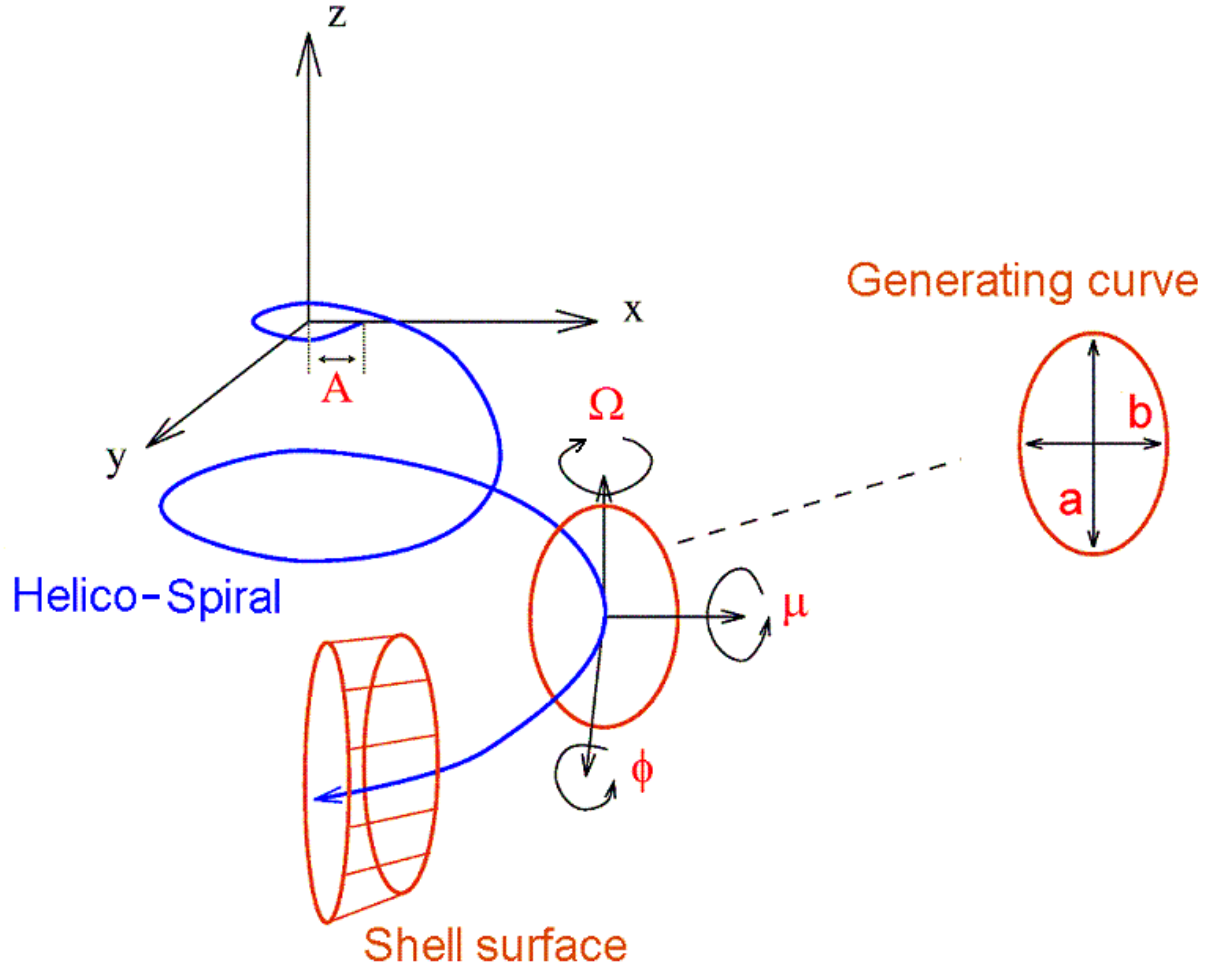
\includegraphics[scale=0.8]{./img/generating_curve_rot.png}
	\caption{3 axes of rotation. \cite{JORGEPICADO}}
	\label{3d-printed-torus} % Unique label used for referencing the figure in-text
	%\addcontentsline{toc}{figure}{Figure \ref{fig:placeholder}} % Uncomment to add the figure to the table of contents
\end{figure}

To get a large final equation:

\begin{equation}
\mathbf{S}'(u,v,s) =
\begin{cases}
	x = D[A sin(v) cos(u) + cos(s + \phi) cos(u + \Omega) \cdot r_c(s) - sin(\mu) sin(s + \phi) sin(u + \Omega)]  e^{u \cot \alpha}\\
	y = [A sin(v) sin(u) + cos(s + \phi) sin(u + \Omega) \cdot r_c(s) + sin(\mu) sin(s + \phi) cos(u + \Omega) \cdot r_c(s)]  e^{u \cot \alpha}\\
	z = [-A cos(v) + cos(\mu)sin(s + \phi) \cdot r_c(s)]  e^{u \cot \alpha}
\end{cases}
\end{equation}


$D$ takes a value of 1 or -1, if the direction of coiling is either dextral or sinistral, respectively. The paper also presents some additional parameters for protrusions. Though they have been implemented in this project, they remained unused since the goal is to use RD textures for such purposes.

\pagebreak

\subsubsection{Processing}
	
Some time was spent trying to get an existing implementation of this equation to work. An existing project used Processing and was abandoned in 2012. It required porting to a new version of Processing and, though an attempt was made to improve it, it remained buggy. It was useful for gaining an intuition of the effect of different variables, but an implementation in Blender could replace all its features.
	
\begin{figure}[h]
	
	\centering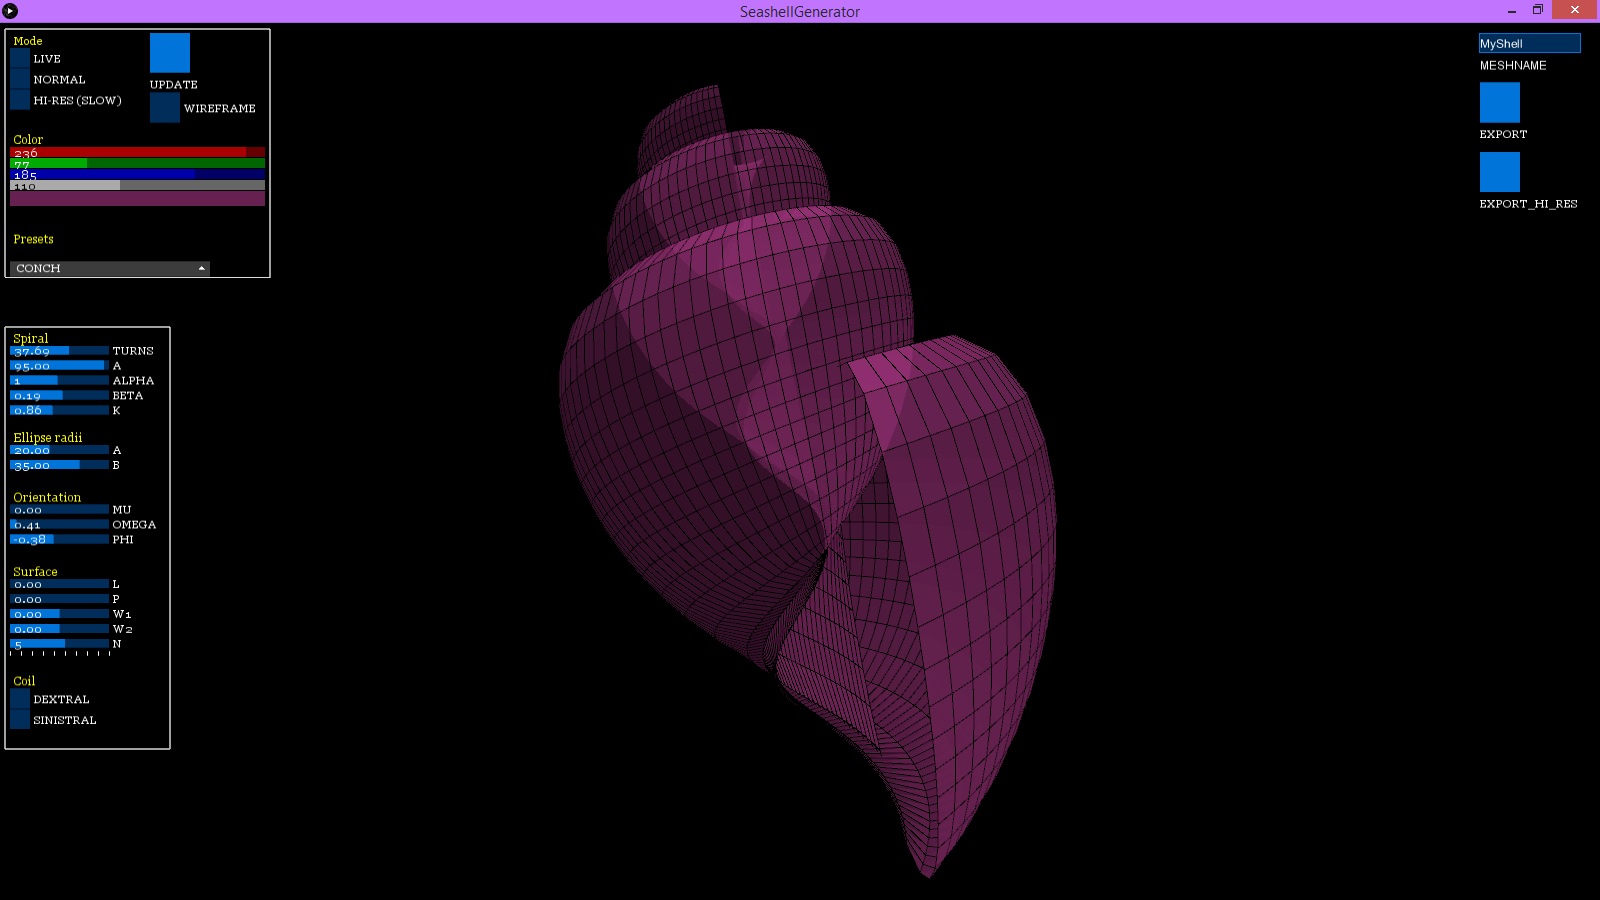
\includegraphics[scale=0.3]{./img/seashell_generator.png}
	\caption{Processing based sea shell generator.}
	\label{activator-inhibitor} % Unique label used for referencing the figure in-text
	%\addcontentsline{toc}{figure}{Figure \ref{fig:placeholder}} % Uncomment to add the figure to the table of contents
\end{figure}

\subsubsection{Blender}

A python script, \textit{blender\_seashell.py},  was created to be used in Blender, which implemented equation (13). After fiddling with the parameters a shell was chosen that resembles hexaplex radix.

\begin{figure}[h]
	\centering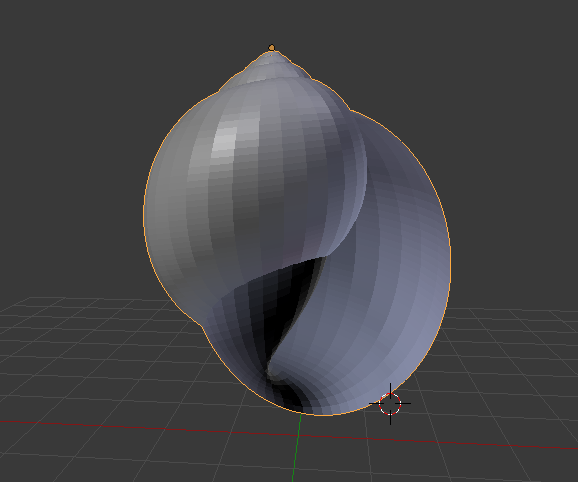
\includegraphics[scale=1.25]{./img/hexaplex_shell.png}
	\caption{Generated by \textit{blender\_seashell.py}.}
	\label{activator-inhibitor} % Unique label used for referencing the figure in-text
	%\addcontentsline{toc}{figure}{Figure \ref{fig:placeholder}} % Uncomment to add the figure to the table of contents
\end{figure}

\pagebreak 

Then it was 3-D printed.

\begin{figure}[h]
	\centering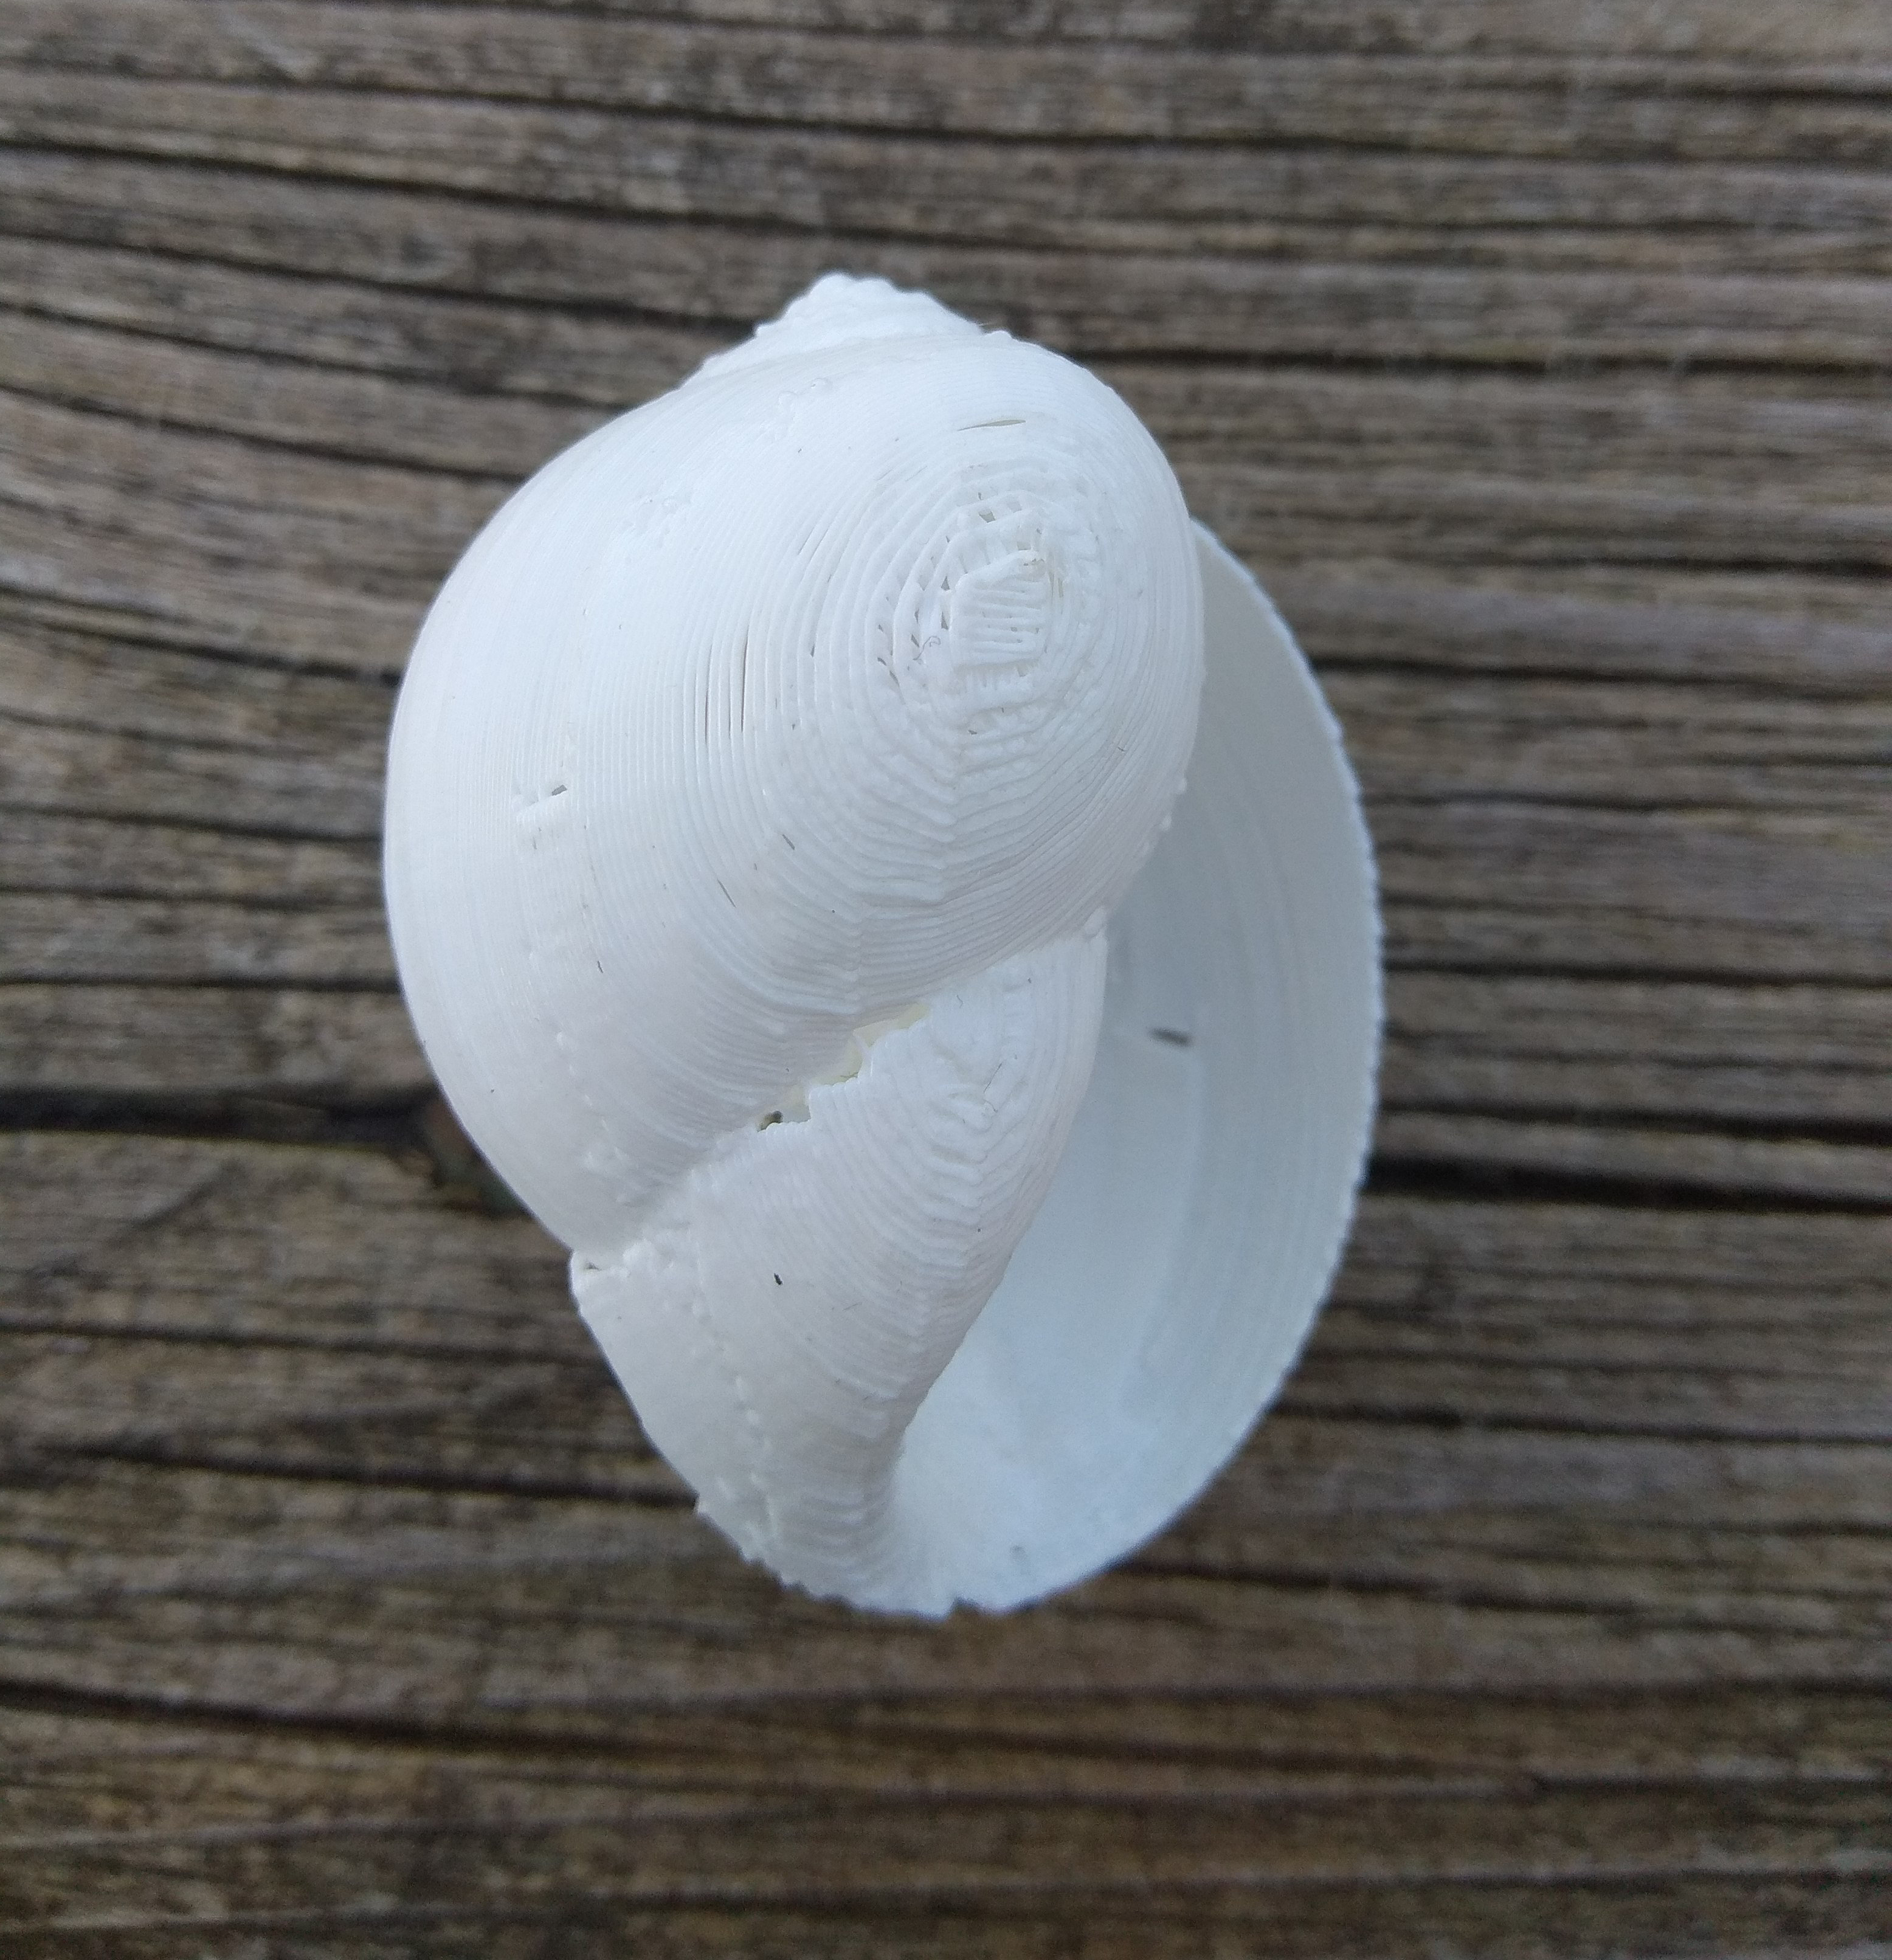
\includegraphics[scale=0.05]{./img/hexaplex_printed.jpg}
	\caption{Printed from \textit{radix\_shell\_only.stl}.}
	\label{activator-inhibitor} % Unique label used for referencing the figure in-text
	%\addcontentsline{toc}{figure}{Figure \ref{fig:placeholder}} % Uncomment to add the figure to the table of contents
\end{figure}


\section{Reaction Diffusion Shaders}

In order to model the protrusion of hexaplex radix an RD texture was created. Notice from Figure 15 that on hexaplex radix the pattern of the protrusions seems to originate from some kind of sinusoidal shape.

\begin{figure}[h]
	\centering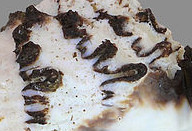
\includegraphics[scale=1.0]{./img/hexaplex_radix_sine.jpg}
	\caption{Sinusoidal pattern on hexaplex radix.}
	\label{hexaplex-sine} % Unique label used for referencing the figure in-text
	%\addcontentsline{toc}{figure}{Figure \ref{fig:placeholder}} % Uncomment to add the figure to the table of contents
\end{figure}

The RD equation used is based on equation 2.4 from \cite{abss}, which uses an activator-inhibitor model.

\begin{equation}
	\frac{\partial a}{\partial t} = \sigma b a^{*2} - r_a a + D_a \frac{\partial^2 a }{\partial x^2}
\end{equation}

\begin{equation}
	\frac{\partial b}{\partial t} = b_b - \sigma b a^{*2} + D_b \frac{\partial^2 b }{\partial x^2}
\end{equation}

\begin{equation*}
	a^{*2} = \frac{a^2}{1+s_a a^2} + b_a
\end{equation*}

\begin{equation*}
\sigma = \rho + r_a  [\tau + \nu \sum_{i=1}^{\eta}{sin(x \cdot rand())}]
\end{equation*}

$a$ represents the concentration of activator and $b$ represents the concentration of inhibitor. $\sigma b a^{*2}$ is the production rate for $a$, and $b_b$ is the production rate for $b$. $-r_a a$ is the depletion of $a$, and $-\sigma b a^{*2}$ is the depletion rate for $b$. $D_a \frac{\partial^2 a }{\partial x^2}$ is the exchange by diffusion. $\sigma$ is mainly a superposition of $sin$ waves to give the pattern a chaotic appearance. This produces a 1-D cellular automata, where the x-axis represents the position and the y-axis represents time.

\begin{figure}[h]
	\centering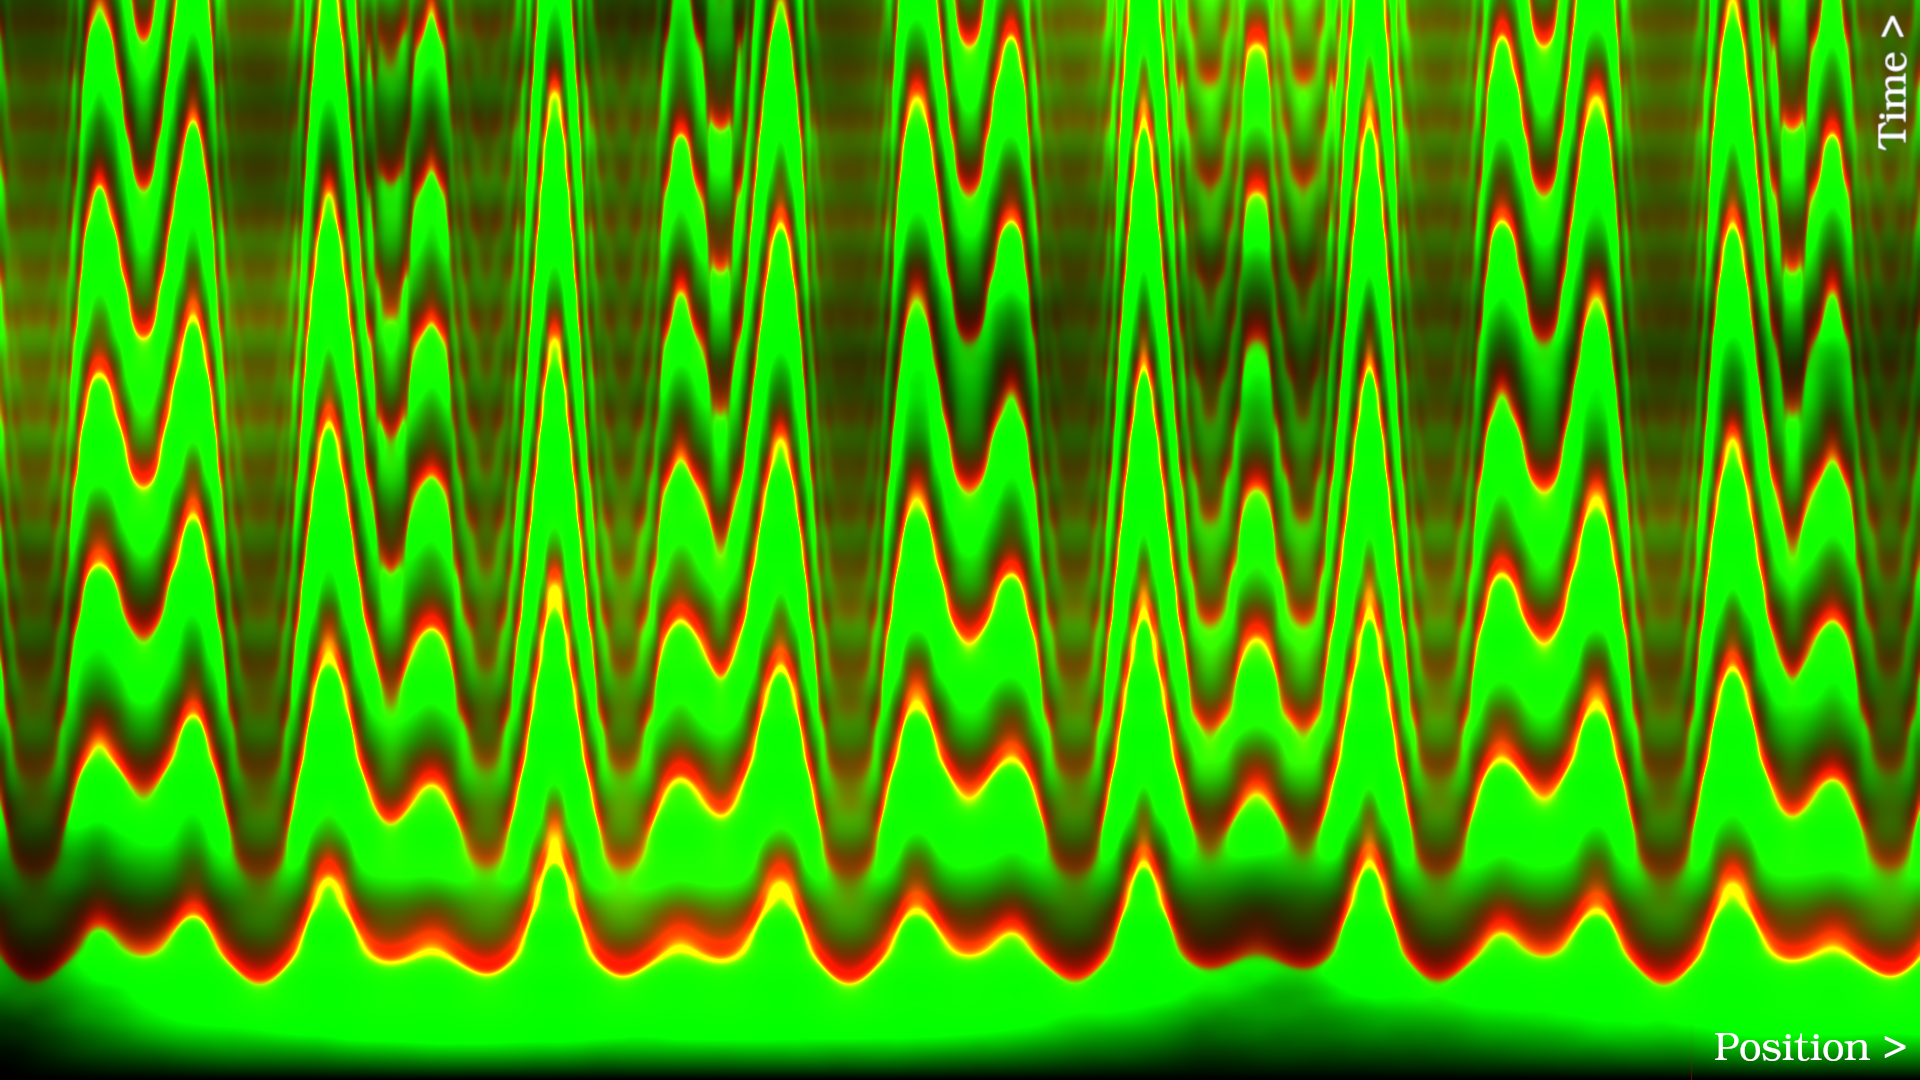
\includegraphics[scale=0.8]{./img/meinhardt-hexaplex-activator-inhibitor.png}
	\caption{Image created from equations (7) and (8). Green value is inhibitor, red is activator. Each value is multiplied by the Fractal Brownian Motion shader. \cite{rd-fbm}}
	\label{activator-inhibitor} % Unique label used for referencing the figure in-text
	%\addcontentsline{toc}{figure}{Figure \ref{fig:placeholder}} % Uncomment to add the figure to the table of contents
\end{figure}

Because the protrusion of hexaplex radix have a mountainous appearance, it seemed appropriate to try adding some fractal noise to the final image. An additional shader was created which multiplies the values of the activator-inhibitor shader by the values of a fractal brownian motion (FBM) texture described in \cite{fbm}. It is difficult to notice in Figure 16, because the RGB values are not clamped to 0 to 1 in the RD shader. Perhaps this should be changed in later attempts.

\begin{figure}[h]
\centering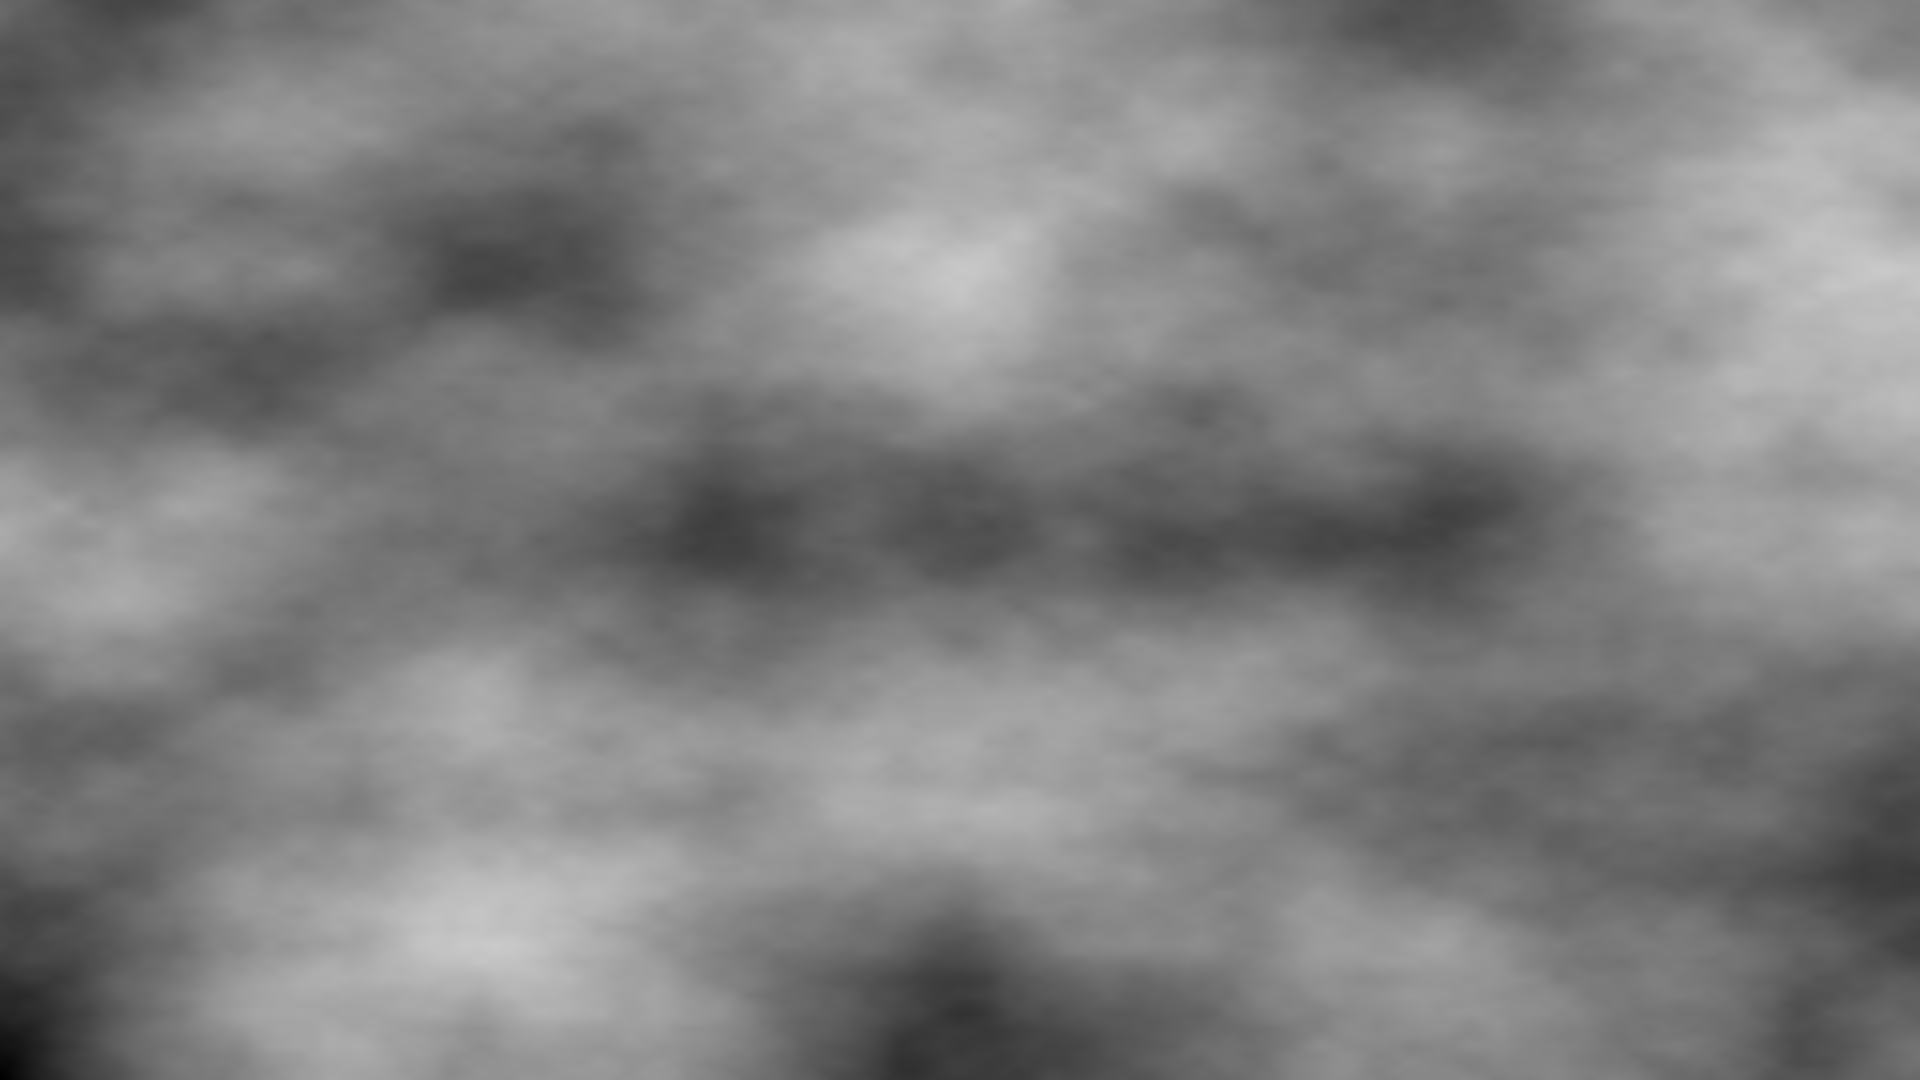
\includegraphics[scale=0.2]{./img/fbm.png}
\caption{Fractal Brownian motion. \cite{st-fbm}}
\label{fbm} % Unique label used for referencing the figure in-text
%\addcontentsline{toc}{figure}{Figure \ref{fig:placeholder}} % Uncomment to add the figure to the table of contents
\end{figure}

Then the activator concentration, red, was converted to the uniform RGB color of the height map texture. 

\begin{figure}[h]
	\centering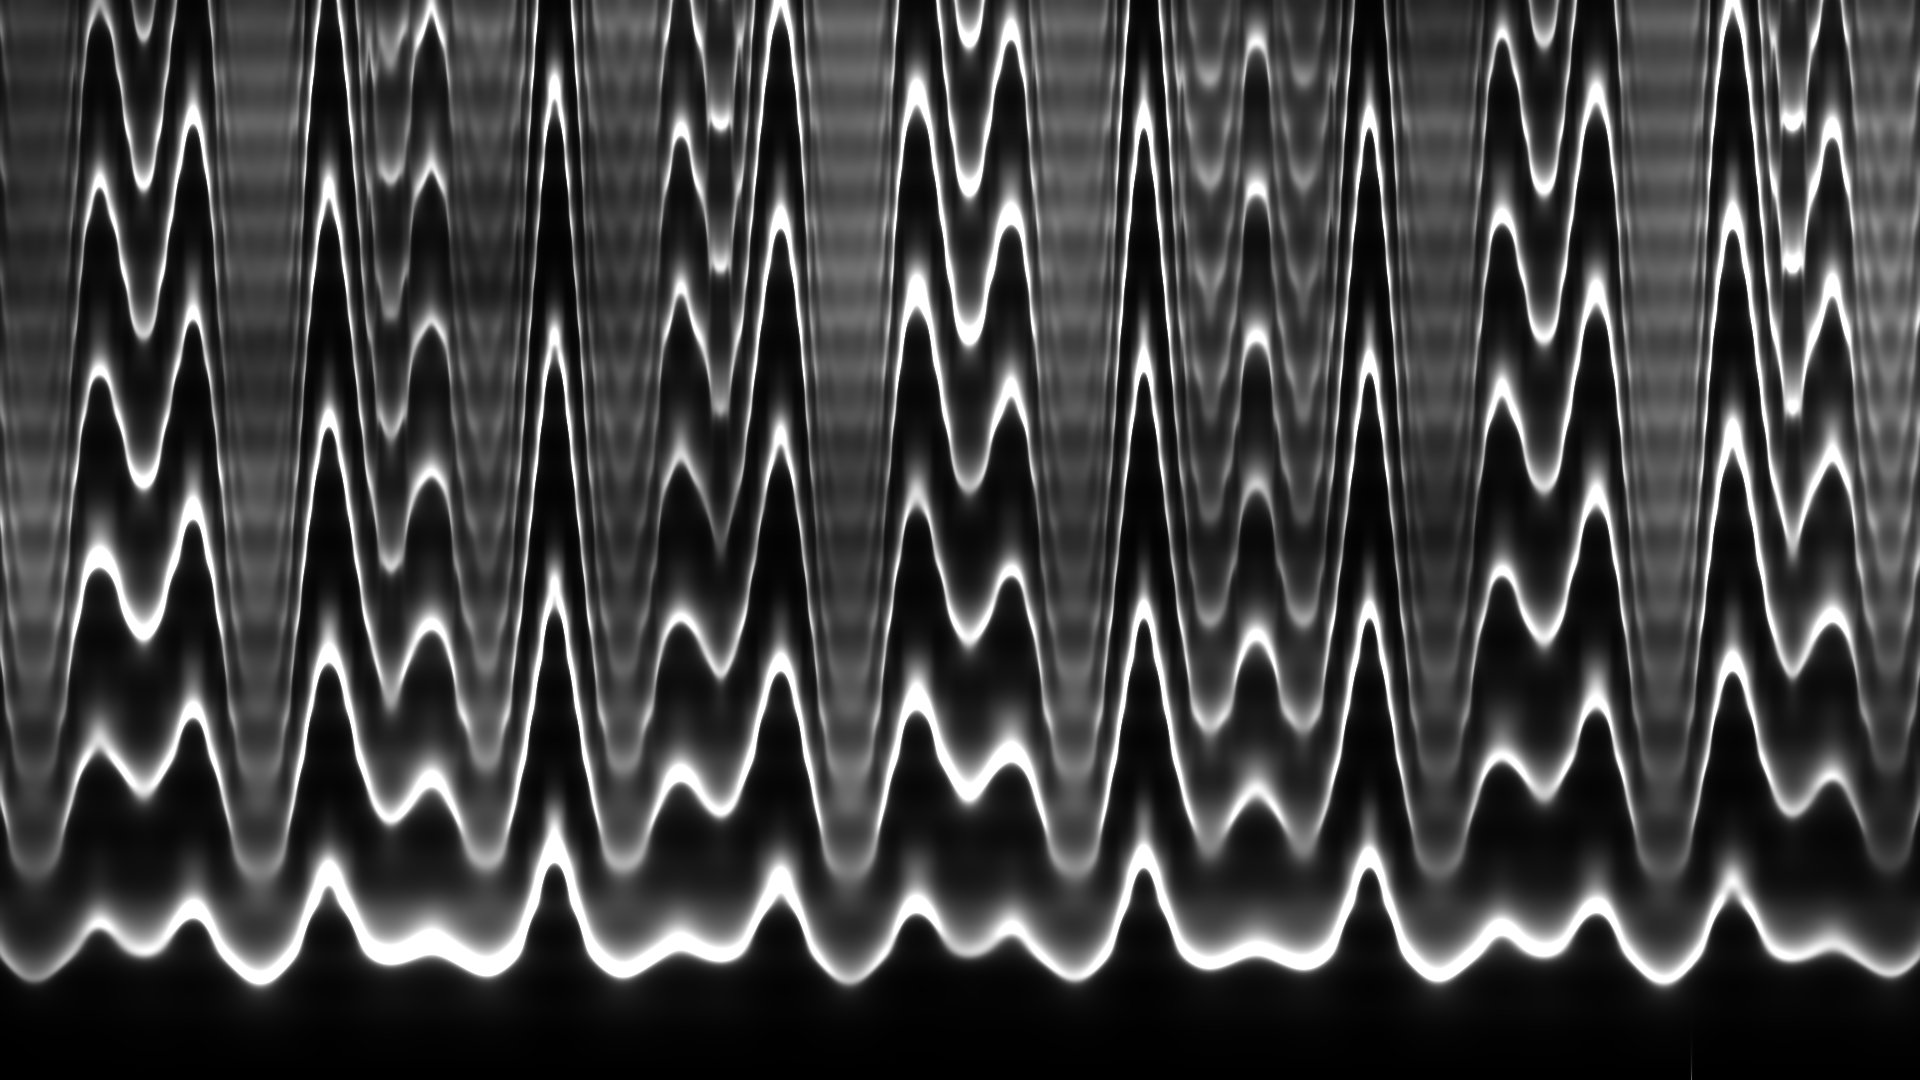
\includegraphics[scale=0.2]{./img/meinhardt-hexaplex.png}
	\caption{Actual height map texture. Red activator value becomes the white color. }
	\label{activator} % Unique label used for referencing the figure in-text
	%\addcontentsline{toc}{figure}{Figure \ref{fig:placeholder}} % Uncomment to add the figure to the table of contents
\end{figure}

\pagebreak


\section{Putting It All Together}

Everything was put together in Blender. The original shell model, seen in Figure 13, was modified so that all non-visible vertices and faces were removed. Then the height map RD texture was UV mapped to the shell. 

\begin{figure}[h]
	\centering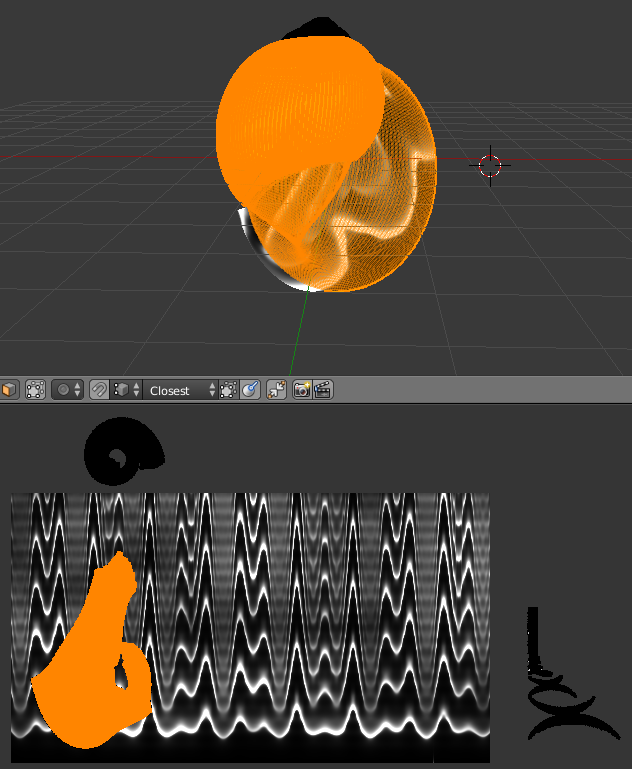
\includegraphics[scale=1.3]{./img/uv_map.png}
	\caption{UV mapping of the texture onto the shell model--.}
	\label{3d-printed-torus} % Unique label used for referencing the figure in-text
	%\addcontentsline{toc}{figure}{Figure \ref{fig:placeholder}} % Uncomment to add the figure to the table of contents
\end{figure}

\pagebreak

Here is the final model in Blender, with the Solidify modifier applied:

\begin{figure}[h]
	\centering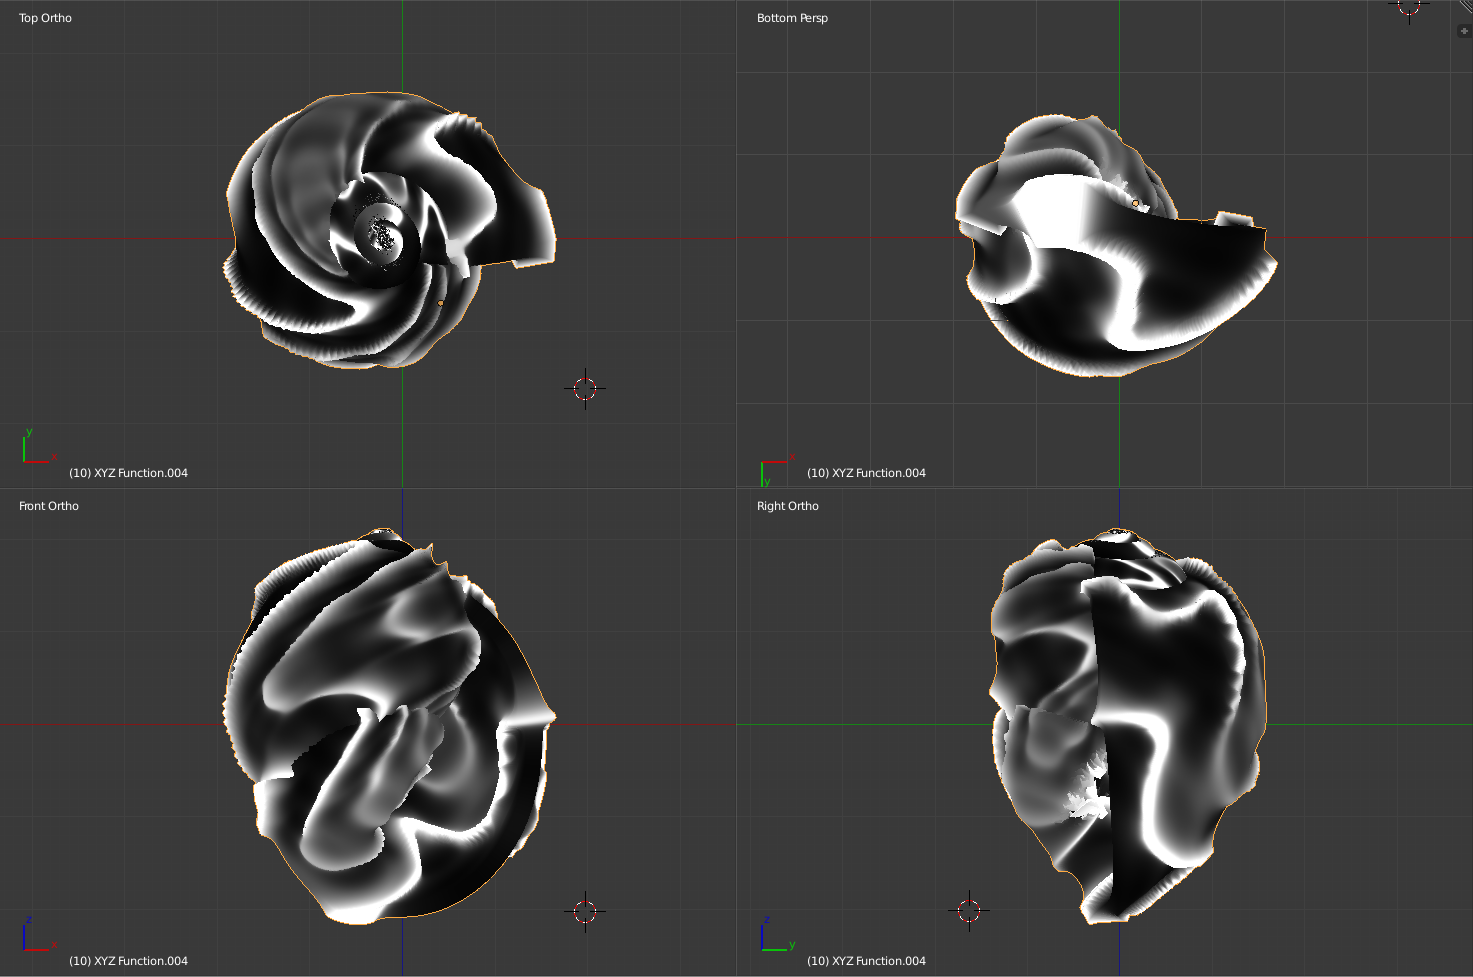
\includegraphics[scale=1.0]{./img/hexaplex_quad.png}
	\caption{Final shell model. \textit{radix\_shell\_textured.stl} contains the geometry of the shell.}
	\label{3d-printed-torus} % Unique label used for referencing the figure in-text
	%\addcontentsline{toc}{figure}{Figure \ref{fig:placeholder}} % Uncomment to add the figure to the table of contents
\end{figure}

I think it looks better with the height map inverted.

\begin{figure}[h]
	\centering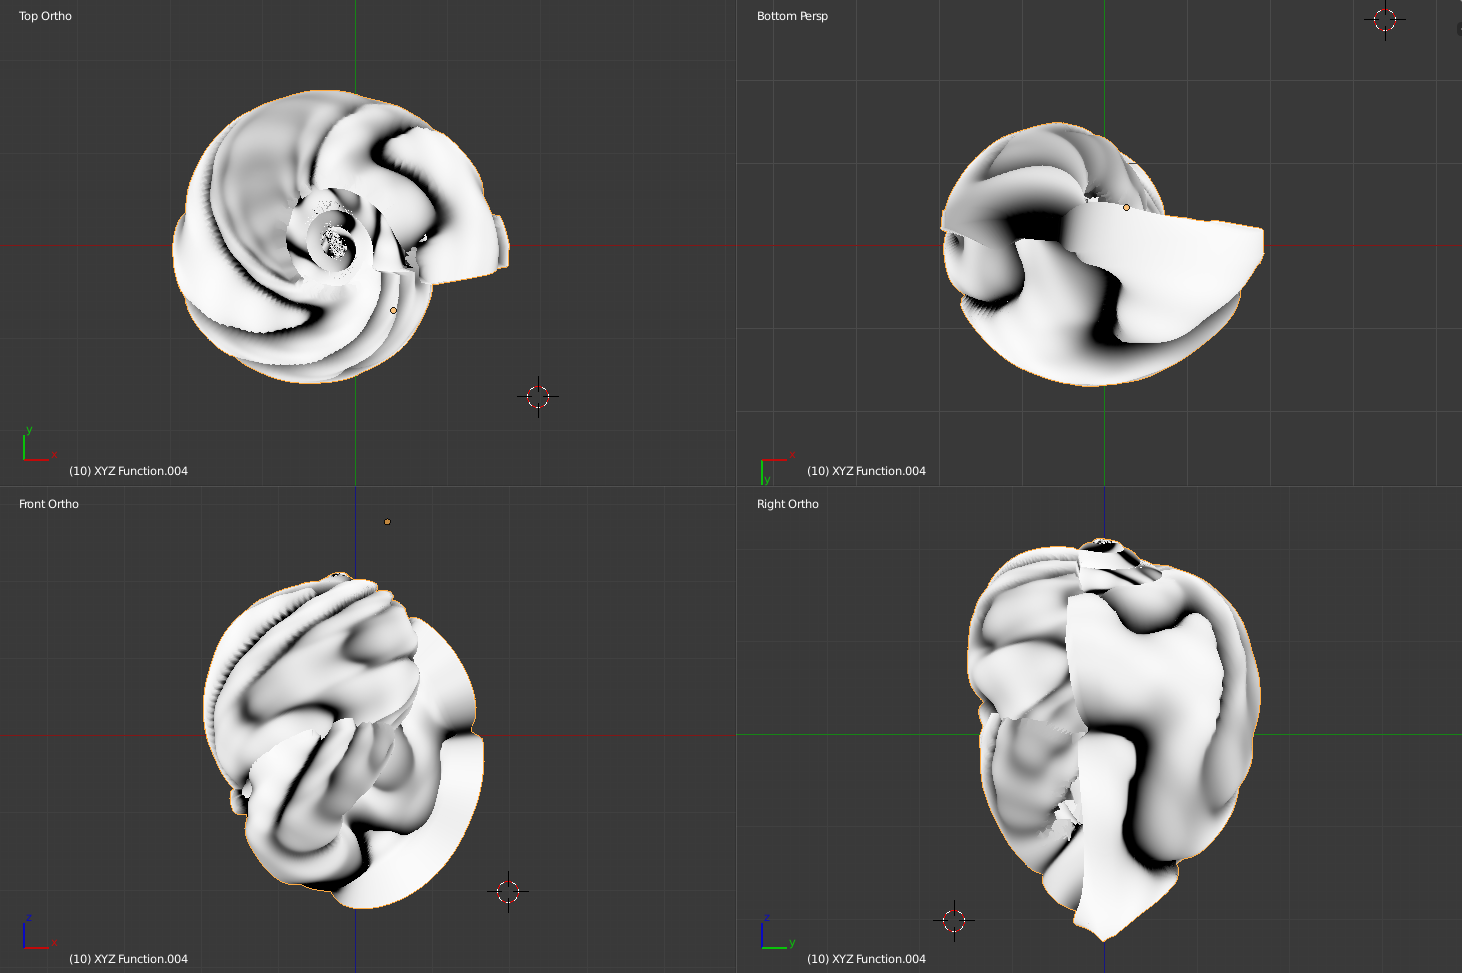
\includegraphics[scale=1.0]{./img/hexaplex_quad_inverted.png}
	\caption{Inverted height map texture applied.}
	\label{3d-printed-torus} % Unique label used for referencing the figure in-text
	%\addcontentsline{toc}{figure}{Figure \ref{fig:placeholder}} % Uncomment to add the figure to the table of contents
\end{figure}

Unfortunately I didn't get to printing the model.

\section{Conclusion}

The striking feature of this project was the change in 3-D modeling technology from the late 1990's. Graphics were likely mostly done using the CPU, so raytracing was dominated rather than meshes, and thus the early project related to creating sea shell models used raytracing techniques. In contrast, application such as Blender can do real-time modification to meshes, which allows for far quicker iteration on equation parameters. Modern tools are also quite general and widely available. It was probably quite a feat for Galbraith et al. to write a CSG library almost 2 decades ago, but modern applications comes with that functionality built in. The trickiest thing about this project hasn't been writing correct software, but rather finding the correct tools and learning how to use them.

As can clearly be seen, there is quite a discrepancy between the intended goal in Figure 1, and the final model in Figure 20. Some small tweaks that may make the resemblance more alike would be to change equations (14) and (15), such that the $sin$ values of $\sigma$ have a higher frequency and smaller amplitude. Doing that in combination with improving the UV mapping such that it fit more correctly would likely improve the similarity between the model and the goal. RD equations can be somewhat unruly and I lack the mathematical dexterity to create new equations that might better model the actual behavior. The UV mapping is also kind of tricky and might require an artistic touch. Also mentioned earlier, it might be a good idea to try to clamp the RD texture's values to a maximum of 1, such that the FBM shader will be more apparent.

Another interesting idea to model the protrusions is to use iterative fractal methods, which could be generalized to produce something like this:

\begin{figure}[h]
	\centering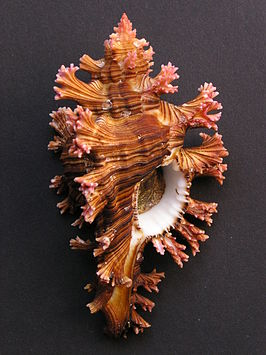
\includegraphics[scale=0.7]{./img/chicoreus_palmarosae.jpg}
	\caption{Chicoreus palmarosae \cite{wikipedia-chicoreus}}
	\label{fig:chicoreus_palmarosae} % Unique label used for referencing the figure in-text
	%\addcontentsline{toc}{figure}{Figure \ref{fig:placeholder}} % Uncomment to add the figure to the table of contents
\end{figure}

\bibliographystyle{plain}
\bibliography{refs}

\end{document}